

\documentclass[man,floatsintext]{apa6}
\usepackage{lmodern}
\usepackage{amssymb,amsmath}
\usepackage{ifxetex,ifluatex}
\usepackage{fixltx2e} % provides \textsubscript
\ifnum 0\ifxetex 1\fi\ifluatex 1\fi=0 % if pdftex
  \usepackage[T1]{fontenc}
  \usepackage[utf8]{inputenc}
\else % if luatex or xelatex
  \ifxetex
    \usepackage{mathspec}
  \else
    \usepackage{fontspec}
  \fi
  \defaultfontfeatures{Ligatures=TeX,Scale=MatchLowercase}
\fi
% use upquote if available, for straight quotes in verbatim environments
\IfFileExists{upquote.sty}{\usepackage{upquote}}{}
% use microtype if available
\IfFileExists{microtype.sty}{%
\usepackage{microtype}
\UseMicrotypeSet[protrusion]{basicmath} % disable protrusion for tt fonts
}{}
\usepackage{hyperref}
\hypersetup{unicode=true,
            pdftitle={Assessing sampling methods for generalization from RCTs: Modeling recruitment and participation},
            pdfauthor={Gleb Furman~\& James E. Pustejovsky},
            pdfkeywords={generalizability, sampling, MRT},
            pdfborder={0 0 0},
            breaklinks=true}
\urlstyle{same}  % don't use monospace font for urls
\usepackage{graphicx,grffile}
\makeatletter
\def\maxwidth{\ifdim\Gin@nat@width>\linewidth\linewidth\else\Gin@nat@width\fi}
\def\maxheight{\ifdim\Gin@nat@height>\textheight\textheight\else\Gin@nat@height\fi}
\makeatother
% Scale images if necessary, so that they will not overflow the page
% margins by default, and it is still possible to overwrite the defaults
% using explicit options in \includegraphics[width, height, ...]{}
\setkeys{Gin}{width=\maxwidth,height=\maxheight,keepaspectratio}
\IfFileExists{parskip.sty}{%
\usepackage{parskip}
}{% else
\setlength{\parindent}{0pt}
\setlength{\parskip}{6pt plus 2pt minus 1pt}
}
\setlength{\emergencystretch}{3em}  % prevent overfull lines
\providecommand{\tightlist}{%
  \setlength{\itemsep}{0pt}\setlength{\parskip}{0pt}}
\setcounter{secnumdepth}{0}
% Redefines (sub)paragraphs to behave more like sections
\ifx\paragraph\undefined\else
\let\oldparagraph\paragraph
\renewcommand{\paragraph}[1]{\oldparagraph{#1}\mbox{}}
\fi
\ifx\subparagraph\undefined\else
\let\oldsubparagraph\subparagraph
\renewcommand{\subparagraph}[1]{\oldsubparagraph{#1}\mbox{}}
\fi

%%% Use protect on footnotes to avoid problems with footnotes in titles
\let\rmarkdownfootnote\footnote%
\def\footnote{\protect\rmarkdownfootnote}


  \title{Assessing sampling methods for generalization from RCTs: Modeling recruitment and participation}
    \author{Gleb Furman\textsuperscript{1}~\& James E. Pustejovsky\textsuperscript{1}}
    \date{}
  
\shorttitle{Assessing sampling methods for generalization from RCTs}
\affiliation{
\vspace{0.5cm}
\textsuperscript{1} University of Texas at Austin}
\keywords{generalizability, sampling, MRT}
\usepackage{csquotes}
\usepackage{upgreek}
\captionsetup{font=singlespacing,justification=justified}

\usepackage{longtable}
\usepackage{lscape}
\usepackage{multirow}
\usepackage{tabularx}
\usepackage[flushleft]{threeparttable}
\usepackage{threeparttablex}

\newenvironment{lltable}{\begin{landscape}\begin{center}\begin{ThreePartTable}}{\end{ThreePartTable}\end{center}\end{landscape}}

\makeatletter
\newcommand\LastLTentrywidth{1em}
\newlength\longtablewidth
\setlength{\longtablewidth}{1in}
\newcommand{\getlongtablewidth}{\begingroup \ifcsname LT@\roman{LT@tables}\endcsname \global\longtablewidth=0pt \renewcommand{\LT@entry}[2]{\global\advance\longtablewidth by ##2\relax\gdef\LastLTentrywidth{##2}}\@nameuse{LT@\roman{LT@tables}} \fi \endgroup}
\usepackage{rotating}
\usepackage{float}

\begin{document}
\maketitle

\hypertarget{introduction}{%
\section{Introduction}\label{introduction}}

The multi-site randomized trial (MRT) has become a common design in educational research, particularly in evaluations of intervention effectiveness. In essence, an MRT is a randomized control trial (RCT) that takes place accross multiple distinct sites (e.g.~geographic locations), with random assignment taking place either at the site or unit level. In education such a design may consist of multiple schools being recruited from one or more districts. Once a sample of sites is recruited, students, teachers, classes or whole schools can be randomly assigned either to receive the intervention (treatment group) or to continue business as usual (control group).

The advantage of an MRT design over a single-site RCT is that it maintains the high level of internal validity via randomized treatment assignment, while also supporting a greater degree of generalizability by introducing cross-site variability. Ostensibly, this allows effect estimates to generalize to a larger population than estimates from a single-site design (Raudenbush \& Liu, 2000). However, the ambiguity of how this larger population is defined, and the overall generalizability of large-scale MRTs, has increasingly come under scrutiny.

Generalizability is a multi-faceted causal inference problem that falls under the purview of external validity. For the purpose of the present study, we narrowly define generalizability as the extent to which a sample represents a well-specified population of interest. In the presense of treatment effect heterogeniety, or variability in response to intervention across persons or sites, estimating sample specific average effects may not be relevant beyond the units in the study. This makes intervention evaluations less informative to policy-makers who seek to make evidence-based decisions in populations that are unrepresented by the study sample.

In this context, inadequate sampling strategies have been shown to be a major threat to generalizability of MRTs. Purposive or non random samples may lead to substantially biased estimates of population level effects (Olsen, Orr, Bell, \& Stuart, 2013; Shadish, Cook, \& Campbell, 2002). Several studies have found substantial differences between schools and districts that participate in large scale randomized trials (Fellers, 2017; Stuart, Bell, Ebnesajjad, Olsen, \& Orr, 2017). Beyond accurate effects estimates, generalizability can also be a question of equity. For instance, these studies have shown that small underserved rural districts are underepresented in RCTs sponsored by Institute of Education Sciences, and therefore are less likely to benefit from federally funded research.

RCTs provide a high level of internal validity as they demonstrate the causality of the impact being estimated. In education research, multi-site RCTs, or multi-site randomized trials (MRTs), are used to inform policy decisions by evaluating intervention impacts on a larger scale. Recruitment and randomization occurs at the organizational level (e.g.~schools), ostensibly increasing the diversity of settings in which the study takes place. In practice, however, the generalizability of MRTs is greatly limited by the sampling method being implemented. This is a major drawback for policymakers who are interested in generalizing treatment effects beyond the sample.

RCTs are commonly used in impact evaluations across many fields. Randomized treatment assignment ensures that estimated effects are causal, thus affording a higher level of internal validity. However, these effect estimates may be sample specific. If treatment effects are heterogeneous, then the impact of an intervention cannot be extrapolated beyond the study sample. This is a limiting feature of RCTs since policymakers seeking to implement interventions will have no way of gauging effectiveness in their population of interest.

Random sampling overcomes this limitation by selecting sites from a well-defined population with some known probability. When used in conjunction with randomized treatment assignment, this is known as dual randomization. Assuming no refusals during recruitment, and full compliance without attrition after assignment, this design enables unbiased estimation of the sample average treatment effect (SATE). Using the known sampling probabilities, the SATE can then be used to estimate the population average treatment effect (PATE).

In absence of random sampling, PATE can still be estimated by using propensity score techniques, provided there is sufficient overlap between the sample and the population (Kern, Stuart, Hill, \& Green, 2016; O'Muircheartaigh \& Hedges, 2014; Tipton, 2013a). This is especially useful in impact evaluation as probability sampling is rarely used in this context (Olsen et al., 2013; Shadish et al., 2002). Instead, researchers often opt for convenience or purposive samples. These methods much less expensive to implement, but are not usually designed for representative sampling. This makes them susceptible to substantial differences between the sample and target population, referred to as under-coverage (Groves, 2004).

Under-coverage can be assessed using several techniques (Stuart, Cole, Bradshaw, \& Leaf, 2011; Tipton, 2014) which identify how well a sample would generalize to a specific population. When under-coverage is too great, the full PATE cannot be recovered with the given sample, and the population needs to be trimmed by removing subsets of sites that are not represented. This can greatly diminish the relevance of study results and undermine the substantial investment into large-scale MRTs.

A series of recent papers instead advocate planning for generalizability at the recruitment stage (Tipton, 2013a, 2013b). These methods require a well defined and enumerated population for which there is extant data, making them especially relevant in the educational context. One method in particular, Stratified Balanced Sampling (SBS), has attracted attention from researchers due to its accessibility. The method involves using cluster analysis to split the population into smaller homogeneous strata and ranking sites within each stratum to prioritize for recruitment in order to achieve a representative sample. Researchers who are interested in using this to sample schools may even use a website (www.thegeneralizer.org) which guides them through this process using data from the Common Core of Data.

Potential advantages of SBS include reducing under-coverage and greater recruitment transparency. However, little methodological work has examined this method's effectiveness. Schools and districts with certain characteristics are unlikely to participate in large-scale MRTs (Fellers, 2017; Stuart et al., 2017; Tipton et al., 2016). If one or more strata are comprised of difficult schools, researchers may resort to convenience sampling within those strata. Furthermore, the additional resources required to recruit from all strata create concerns regarding practicality.

The goal of the current paper is two-part. First, we propose several methods for modeling two major sources of sampling bias: recruitment and participation. Recruitment refers to how likely a sampling site is to be approached by researchers, and participation refers to how likely the sampling site is to participate if recruited. This step will lay the groundwork for testing sampling methods in the educational context. Second, using the models proposed in the first step, we will compare SBS to several other recruitment models on the method's ability to select a generalizable sample, and the ease with which a full sample can be recruited.

\hypertarget{stratified-balanced-sampling}{%
\section{Stratified Balanced Sampling}\label{stratified-balanced-sampling}}

In this section we demonstrate SBS within the context of selecting schools for a large-scale MRT. This application will also serve as the basis for the present simulaion study which will be further outlined in a later section. SBS is a flexible method that is adaptable to various data sets and, depending on study circumstances and design, may require different strategies or methods than presented here. For a more complete consideration of SBS, see Tipton (2013b).

SBS applies cluster analysis as a dimension reduction technique to drive bias-robust balanced sampling based on a large set of covariates. The ultimate goal is to select a sample that is representative of a population along a set of covariates related to treatment heterogeneity and site participation. This process requires the availability of a rich data set of observed covariates for each site in the population. We therefore begin by discussing the data which will serve as the sampling frame and the covariates we have selected.

Following recomendations proposed by Tipton (2013b), we then implement k-means clustering to divide the population into heterogeneous strata comprised of homogeneous sites. K-means clustering assigns sites to strata such that similarity within each stratum is maximized. This step requires us to specify the number of strata that need to be generated. Here we rely on both empirical criteria as well as subjective appraisals of what is feasible to implement.

After determining the strata, we then use a second distance metric to rank sites in order of how representative the site is of its stratum. These ranks are later used to drive \enquote{balanced sampling} by prioritizing sites for recruitment. In practice, these rankings should encourage the selection of sites from subsections of the population which may otherwise not have been included given typical sampling strategies.

Finally, we discuss the advantages and limitations of SBS given our implementation, and the potential difficulties of using this to sample schools in the greater context of educational research.

\hypertarget{sample-frame}{%
\subsection{Sample Frame}\label{sample-frame}}

We first identify a population of schools from which we want to select a representative sample. Six States served as the geographic boundries for this sample frame: California, Oregon, Pensilvania, South Carolina, Texas, and Wyoming. These six states were selected for arbitrary reasons, \textbf{\emph{blah blah blah}}.

The cluster analysis requires data to enumerate all population units and provide key characteristics that are hypothesized to mediate treatment heterogeneity. Since we are only interested in selecting a representative sample, we instead identified covariates that predict school participation in RCTs. Our goal here is for our final sample to include schools not normaly found in large-scale evaluations of interventions. To this end, selection of covariates was driven by prior research on district and school participation behavior in RCTs (Stuart et al., 2017; Tipton et al., 2016a; Fellers, 2017). These studies found that districts and schools with higher proportions of students who are English language learners (ELL), economically disadvantaged (ED), non-White, and living in urban settings are more likely to participate, as are larger districts and schools.

It is important to note, however, that some of these characteristics might also make it more likely that researchers would recruit these districts and schools in the first place. That is to say, school characteristics may drive selection bias by both impacting the types of schools that agree to participate, as well as by the types of schools that researchers recruit. For instance, the overrepresentation of larger schools in RCTs can mean that schools with more students are more likely to agree to participate, are more likely to be recruiterd by researchers, or a combination of both. Therefore, the participation behavior outlined here is likely not representative of all schools in the US, rather only schools that are likely to be recruited by current practices.

Characteristics of the sample frame were sourced from the Common Core of Data (CCD; \url{https://nces.ed.gov/ccd/index.asp}). The CCD is a comprehensive database housing annually collected census of all public schools and districts. Log-transformation was used on school size (number of students), district size (number of schools) and the student to teacher ratio. This is done to allow proportional comparisons at the extremes of the distributions (Hennig \& Liao, 2013). For instance, the difference between two schools with 4000 and 3000 students should be weighed as much as the difference between two schools with 400 and 300 students when generating clusters. Figure \ref{fig:plot-dist1} displays the distribution of the continuous variables used. Two categorical covariaets were used as well: urbanicity (urban, suburban, or town/rural) and a binary indicator of school wide title 1 elegibility. In all, the sample frame consists of 6 states, 2,016 districts and 9,792 schools.



\begin{figure}
\centering
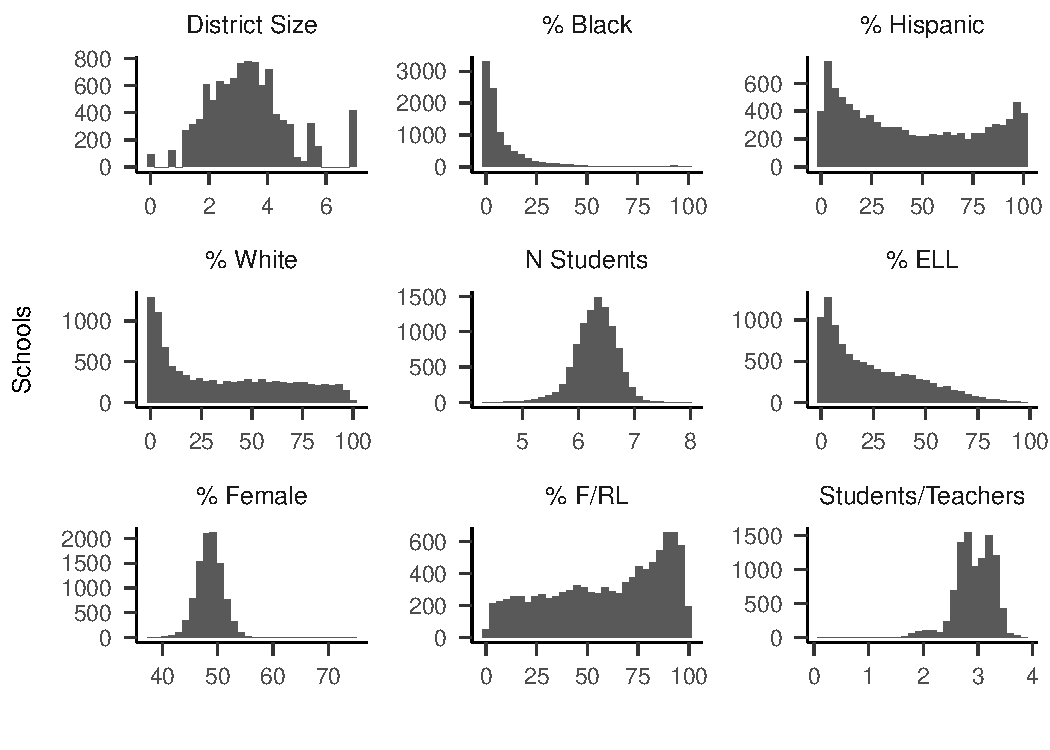
\includegraphics{GenSamp-Paper_files/figure-latex/plot-dist1-1.pdf}
\caption{\label{fig:plot-dist1}Distributions of continous covariates. Three covariates were transformed to logs: (1) District Size, (2) N Students, and (3) Student/Teachers}
\end{figure}

\hypertarget{stratification}{%
\subsection{Stratification}\label{stratification}}

Stratification was performed prior to simulation because the population is constant across iterations. Per Tipton (2013b)'s original recommendation, we use k-means clustering to partition the population into strata. This requires selecting a distance metric, choosing the number of strata, and generating the strata. All analyses were performed in R (R Core Team, 2018).

\hypertarget{cluster-analysis}{%
\subsubsection{Cluster Analysis}\label{cluster-analysis}}

We performed the cluster analysis using the \emph{cluster} package (Maechler et al., 2017). First, the \emph{daisy} function is used to compute an \(n\) by \(n\) pairwise distance matrix across all observations. This function requires two parameters: (1) the data matrix, and (2) the distance metric. The data matrix includes the full set of school level covariates used to compare schools for clustering. The distance metric selected for this analysis largly depends on the type of data in the matrix.

The distance metric summarises the difference between a pair of sites on a set of covariates in order to maximize the similarity of all sites within a cluster. In educational research, as is the case here, data are likely to contain both continuous and categorical variables. For mixed data such as this it is appropriate to use the general similaity measure (Gower, 1971; Tipton, 2013b).

This measure relies on different calculations of distance depending on the type of covariates. Let \(X_{hi}\) and \(X_{hi'}\) be the observed value of covariate \(h = {1, ..., P}\) for sites \(i\) and \(i'\) respectively, where \(i \ne i'\). Let \(d_{ii'h}\) be the distance between observed values of covariate \(X_{h}\) for site \(i\) and site \(i'\). For categorical or dummy coded variables, \(d_{ii'h} = 1\) if \(X_{hi} = X_{hi'}\) and \(d_{ii'h} = 0\) otherwise. For continuous covariates, we use the following formula:

\begin{align}
  d_{ii'h} = 1 - \frac{|X_{hi} - X_{hi'}|}{R_h}
\end{align}

where \textbar{}.\textbar{} indicates absolute value, and \(R_h\) is the range of observations for covariate \(X_h\). This equation restricts the range of \(d_{ii'h}\) to \([0,1]\). Finally, we calculate the general similarity between each site pair by taking the weighted average of the distances between all covariates. Let \(d^{g}_{ii'}\) be the general similarity between site \(i\) and site \(i'\).

\begin{align}
  d^{g}_{ii'} = \frac{\sum^p_{h = 1}w_{ii'h}d_{ii'h}}{\sum^p_{h = 1}w_{ii'h}}
\end{align}

where \(w_{ii'h} = 0\) if \(X_h\) is missing for either site and \(w_{ii'h} = 1\) otherwise. Setting the distance metric to \enquote{gower} in the \emph{daisy} function performs these calculations.

\hypertarget{number-of-strata}{%
\subsubsection{Number of Strata}\label{number-of-strata}}

Next we used the \emph{kmeans} function to generate clusters, which employs an optimization algorithm to classify sites into \(k\) clusters by minimizing the total within cluster variance. For each \(k\), it is recommended to run \emph{kmeans} at least 10 times, and select the clustering that results in the smallest total within-cluster sum of squares. This function also requires two parameters: (1) the distance matrix from the previous step, and (2) the number of clusters to generate (\(k\)).

Selecting an appropriate value for \(k\) is one of the most difficult problems in cluster analysis (Steinley, 2006). Tipton (2013b) states that both empirical and practical criteria should be used in selecting \(k\). A larger set of strata would result in greater homogeneity within each stratam, however it may also be more difficult to manage for recruiters. For instance, if refusal and non-response rates are fairly high, having fewer sites spread across more strata may make it difficult to adequately recruit from all strata. Resource constraints (e.g.~time, funding, recruiters) may also be a factor in the number of strata selected.

Hennig and Liao (2013) also argue that the method of selecting \(k\) should depend on the context of the clustering, framing the issue as one of obtaining an appropriate subject-matter-dependent definition rather than a statistical estimation. With considerations in mind, we examined three criteria: (1) a generalized form of the Calinski-Harabasz index (Cali\a'nski \& Harabasz, 1974) proposed by Hennig and Liao (2013), (2) the proportion of between-cluster variance as recommended by Tipton (2013b), and (3) the practicality of sampling from fewer clusters.

Our strategy was to perform the analysis several times- generating different numbers of strata- and comparing all performance criteria for each number of strata generated (Figure \ref{fig:fig-k-plots}). We first calculated the Calinski-Harabasz (CH) index using the \emph{cluster.stats} function from the \emph{fpc} (Hennig ???) package. Figure \ref{fig:fig-k-plots}a displays the CH index for each \(k\) clusters generated. In this case, generating 2 clusters maximises the CH-index.

The proportion of between-cluster variance was calculated manually. Let \(k\) be the number of strata generated where \(k = 1, 2, ..., q\) for some maximum allowable number of \(q\) strata. Let \(\sigma_{wk}^2\) be the total variability within each stratum, and \(\sigma_{bk}^2\) be the total variability between each stratum, for all covariates in \(X\) and for each set of \(k\) strata generated. Let \(p_k\) be the proportion of variability that is between strata for each set of \(k\) strata generated be defined as follows:

\begin{align} \label{eq:pk}
  p_k = \sigma_{bk}^2/(\sigma_{wk}^2 + \sigma_{bk}^2)
\end{align}

As \(p_k\) approaches 1, most of the variation is between strata, indicating homogeneity within strata. This increases the possibility of selecting a more balanced sample. Figure \ref{fig:fig-k-plots}b plots \(p_k\) against \(k\)m allowing visual comparison of the results. The \(k\) for which the rate of change \(p_k\) slows is considered favorable. Tipton (2013b) also recommends selecting the number of clusters such that at least 80\% of the variability is between clusters, indicated by the figure as a dashed line. Given this criteria it seems that at least 7 clusters should be generated. However we also see that after a sharp initial increase, the slope of the graph begins to level out. This indicates that as we increase the number of clusters, the benefit of doing so decreases, while the difficulty of sampling from each cluster increases. In that case after 5 or 6 clusters the difficulty of sampling may not be worth such small increases in homogeneity within clusters.

Figure \ref{fig:fig-k-plots}c plots the sample size that needs to be selected from each cluster to fulfill the proportional allocation requirement such that the number of sites sampled from each cluster is proportional to the size of the cluster in the population. The dashed line indicates the ideal allocation if all clusters were of equal size. We see that the variability in cluster sizes decreases as more clusters are generated. A sensible cutoff may be determined by looking at the size of the smallest cluster. At \(k > 8\) it seems that the smallest clusters would require less than 5 sites being sampled, which may be very difficult in a practical setting. We determined that this would be the most likely criteria to be conisdered in the field, and ultimately decided to generate 5 clusters for this analysis.









\begin{figure}
\centering
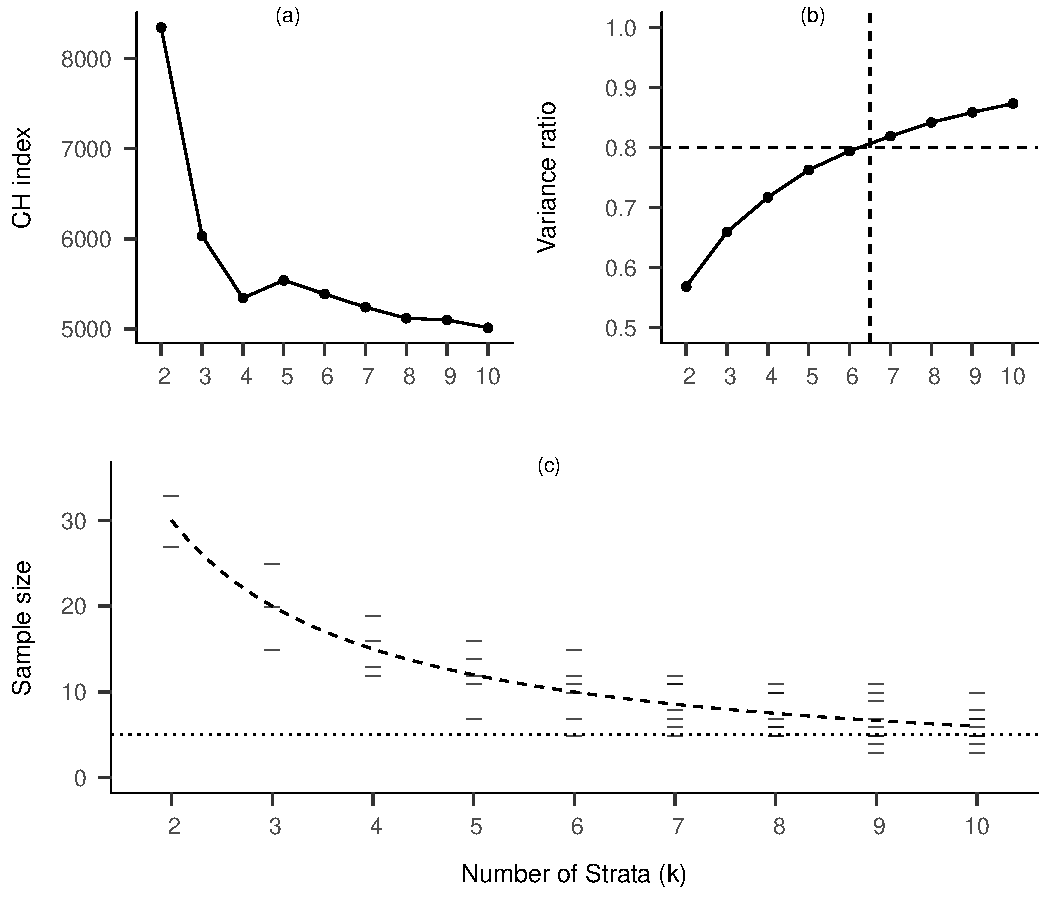
\includegraphics{GenSamp-Paper_files/figure-latex/fig-k-plots-1.pdf}
\caption{\label{fig:fig-k-plots}Plots used to determine value for \(k\). (\emph{a}) Calinski-Harabasz index - peaks indicate better fit. (\emph{b}) Ratio of between cluster sum of squares to total cluster sum of squares - horizontal line indicates cutoff of .8, vertical line indicates minimum number of clusters needed to achieve cutoff. (\emph{c}) Sampling requirements for each cluster given proportional alocation - horizontal line indicates a cluster sample size requirement of 5 schools.}
\end{figure}

\hypertarget{balanced-samplingo}{%
\subsection{Balanced Samplingo}\label{balanced-samplingo}}

The goal of balanced sampling is to recruit in such a way that the expected value of covariate \(X_h\) across sites in stratum \(j\) is equal to the expected value of covariate \(X_h\) across all sites sampled from stratum \(j\):

\begin{align}
  E(X_ih|Z_i = 1, j) = E(X_h|j)
\end{align}

where \(Z_i = 1\) if site \(i\) is recruited into the sample and \(Z_i = 0\) otherwise. Following Tipton (2013b), we implemented balanced sampling by prioritizing the recruitment of sites based on their similarity to the \enquote{average} site in each stratum. First we identified the number of sites to be sampled from each stratum using proportional sample allocation. Each stratum contains \(N_j\) sites where \(N_1 + N_2 ... + N_k = N\). From each stratum \(j\), we calculated the number of sites to be sampled, \(n_j\), such that \(n_j = [(N_j/N)n]\), where {[}.{]} indicates that each value is rounded to the nearest integer.

Next we ranked each site within a stratum using a distance measure, with sites closer to the \enquote{center} of the strata ranked higher. We calculated the weighted Euclidean distance to the mean of each covariate:

\begin{align} \label{eq:euclid}
  d_{ij} = \sqrt{\sum^p_{h=1}w_h[X_{hij} - E(X_h|j)]^2}
\end{align}

where \(w_h\) is the weight assigned to covariate \(X_h\), \(E(X_h|j)\) is the population mean of covariate \(h\) in stratum \(j\), and \(X_{hij}\) is the value of covariate \(h\) for site \(i\) in stratum \(j\). As with generating the strata, different weights can be used such that distances depend more heavily on covariates thought to be more related to treatment effect heterogeneity. We then used the ranked list to prioritize sites for recruitment, beginning with the highest ranked sites. If a site was unavailable or refused to participate, a recruitment attempt was made with the next highest ranked site until \(n_j\) sites agreed to participate.

\hypertarget{advantages-and-limitations}{%
\subsection{Advantages and Limitations}\label{advantages-and-limitations}}

SBS has only recently proposed and there have not been any large scale implementations of this method reported. Also, beyond the original proposal article, there have not been any methodological investigation into the method. Tipton (2013b) illustrated SBS by comparing it to a previous study which did not use a formal sampling method (Roschelle et al., 2010). Data from the previous study was used to generate two hypothetical samples. The first sample was the ideal in which the highest ranked schools in each stratum agreed to participate. The second sample was a \enquote{worst case} non-response sample where the first 50 highest ranked schools in each stratum refused to participate, resulting in a non-response rate of at least 83\% in each stratum. These two samples were then compared to the original sample on the first 3 moments of 26 covariates. Both samples achieved with SBS resulted in better balance than the original sample on at least 19 of the 26 covariates in the first two moments, and 14 out of 26 in the third moments. The samples were then compared on how well they would generalize using the method proposed by Stuart et al. (2011). This final test showed that the samples achieved with SBS resulted in less coverage errors than the original sample and would thus be easier to generalize using the retrospective methods.

Stratified sampling methods offer three key advantages: transparency, non-response analysis, and integration with and improvement of post hoc adjustments. Perhaps the most appealing advantage of this method is the transparency it requires of the recruitment process. Researchers are forced to provide clear documentation and reasoning for targeting sites for recruitment. This allows for a more careful critique of the study and a better justification of the recruitment process for funders and other stakeholders. It also allows for a better analysis of non-responders. By identifying a set of observed covariates which may predict treatment heterogeneity prior to conducting the study, non-responders or refusals can be tracked and later analyzed for any systematic differences from the inference population or study participants. Finally, implementing this method does not preclude the use of the retrospective methods previously discussed. SBS may not alleviate all balancing issues, and additional statistical adjustments may need to be made. Even if balance is only partially improved at the sampling stage, coverage errors will still be reduced and less of the inference population will need to be discarded.

There are, of course, several limitations as well. As with the retrospective methods, SBS depends on the existence of a rich set of observed covariates related to treatment heterogeneity and sample selection for each site in the population. Most readily available data sets primarily consist of demographics and may not contain all of the covariates related to variation in treatment effect, which can result in omitted variable bias (Tipton, 2013b). Additionally, SBS requires more resources to implement than a simple convenience sample. Recruiting ranked sites from multiple strata requires a coordinated effort between recruiters (Tipton, Hallberg, Hedges, \& Chan, 2017). This means that recruiters cannot work independently and must rely on a partnership with researchers implementing this method.

Although the findings in Tipton (2013b) were promising, it is unclear how generalizable they are to other potential studies. The inference population consisted of 1,713 non-charter schools serving seventh graders in Texas. Of these schools, 73 (4.3\%) were selected into the sample across nine strata. In other applications, the inference population may be much larger and more heterogeneous, requiring more strata to be created. Sampling from too many strata is difficult when sample sizes are restricted. Would this method be beneficial to researchers making inferences on a national scale? In order to create a non-response condition, Tipton (2013b) selected the first 50 sites in each stratum to be refusals, resulting in smaller strata having higher non response rates.

Furthermore, what if schools in larger strata had higher non-response rates? How many schools would recruiters have to contact before collecting a full sample? School recruitment is a time consuming and complicated process which requires approval at several levels. Researchers may not want to invest in recruiting schools from strata with particularly high non response rates. Finally, the data came from a single state which happened to provide information on 26 covariates. If a national population was of interest, more states would need to be included, but data reporting is not uniform across all states.

\hypertarget{simulation-study}{%
\section{Simulation Study}\label{simulation-study}}

In this section we describe the simulation study developed to assess the generalizability of the samples selected by SBS relative to several other sampling methods, and the feasibility with which the sampling methods can be employed. Real data was used to inform the sample frame.
Selection bias was generated to account for both self selection as well as researcher bias.

\hypertarget{methods-and-models}{%
\section{Methods and Models}\label{methods-and-models}}

\hypertarget{framework-for-generalizability}{%
\subsection{Framework for Generalizability}\label{framework-for-generalizability}}

We begin with a data set enumerating a population of \(N\) sites (schools), indexed as \(i = 1 ... N\). We assume that each site has some unobserved probability of participating in a study if approached by recruiters which is represented by the participation propensity score \(\pi_i^P\). Each site also has a vector of observed characteristics \(X_i\) of length \(P\). This is a set of pre-treatment covariates that predict \(\pi_i\). The covariates are a mixture of continuous, binary, and categorical data.

The goal is to select a sample of \(n\) sites such that there is balance along \(X_i\) between the sample and the population, indicating that the population is fully represented by the sample. We measure balance using the standardized mean difference (\(SMD\)) between the sample and population for a given covariate. \(SMD\) is calculated as

\begin{align}
  SMD = \frac{\bar{X}-\mu}{\sigma}
\end{align}
where \(\bar{X}\) is a vector of covariate means in the sample, \(\mu\) is the vector of covariate means in the population, and \(\sigma\) is the vector of covariate standard deviations in the population. \(SMD\) values closer to zero indicate greater balance between the sample and the population.

\hypertarget{modeling-selection-bias}{%
\subsection{Modeling Selection Bias}\label{modeling-selection-bias}}

Selection bias stems from two sources: (1) site participation behavior and (2) researcher recruitment behavior. To model the former we propose a simple participation propensity score. Let \(\pi^P_i\) represent the participation propensity score, or the probability that a site agrees to participate in an RCT if approached for recruitment. Using a simple logistic transformation we model \(\pi^P_i\) as follows:

\begin{align} \label{eq:RGM}
  log\bigg(\frac{\pi^P_i}{1 - \pi^P_i}\bigg) = \beta_0 + \boldsymbol{X_i \beta}
\end{align}
where \(\boldsymbol{X_i}\) is an \(N\) by \(P\) matrix of covariates that predict sample selection for each site, and \(\boldsymbol{\beta}\) is a vector of coefficients associated with those covariates. Participation for site \(i\) will be determined by sampling from a Bernoulli distribution with probability equal to \(\pi^P_i\).

To generate selection bias stemming from researcher recruitment, we propose a \enquote{low hanging fruit} approach to convenience sampling. We assume that researchers have some knowledge of how likely each site is to participate, and prioritize easy to recruit sites as a way of maximizing recruitment efficiency. While there are many other ways to define convenience sampling, we posit this as a first step. Sites are prioritized for recruitment by sequentially sampling from the population of sites using \(\pi^P_i\) as a sampling weight. Once a site is added to the list in order of priority, the probability of choosing the next site is proportional to the weights of the remaining items. In this way, sites that have higher values for \(\pi^P_i\) are more likely to be recruited earlier on.

\hypertarget{participation-propensity-score}{%
\subsubsection{Participation Propensity Score}\label{participation-propensity-score}}

A response generating model (RGM) was developed to simulate self selection. The RGM creates a propensity score for each school that indicates the probability of the school agreeing to participate if targeted by any of the sampling methods. This model assumes that schools can be recruited directly by researchers. Recall equation \eqref{eq:RGM} where \(\pi^P_i\) is generated for each site \(i\) using a linear tranformtion of the observed covariates with a logit link function. The set of covariates, \(X_i\), was composed of variables described above. The corresponding coefficients, \(B\), were based on work by Fellers (2017) who compared 571 elementary schools that participated in IES funded studies to the full population of U.S. elementary schools. Absolute SMD between the schools that participated and the population were reported. By standardizing \(X_i\) and using the reported SMDs as coeficients, we generated \(\pi^P_i\) values that should on average mimic the samples that Fellers studied.

Intercept values were manipulated to generate different levels of population participation rates. Since these rates are unknown, we selected parameters for 9 levels of participation rates. Table \ref{tab:tab-RGM-Pars} reports the variables, variable codes, and coeficients used in the RGM. Covariate coefficients remained constant across response rates.

\begin{table}[tbp]
\begin{center}
\begin{threeparttable}
\caption{\label{tab:tab-RGM-Pars}Ods ratio coefficients for Response Generating Model}
\begin{tabular}{ll}
\toprule
Variables & \multicolumn{1}{c}{log\_odds}\\
\midrule
District Size & 0.52\\
\% Black & 0.29\\
\% Hispanic & 0.40\\
\% White & -0.54\\
N Students & 0.37\\
\% ELL & 0.41\\
\% Female & -0.02\\
\% F/RL & 0.08\\
Students/Teachers & -0.10\\
Suburban & 0.01\\
Schoolwide Title I & 0.02\\
Town/Rural & -0.40\\
Urban & 0.43\\
\bottomrule
\end{tabular}
\end{threeparttable}
\end{center}
\end{table}



\hypertarget{sampling-methods}{%
\subsection{Sampling Methods}\label{sampling-methods}}

Five sampling methods were compared: stratified and unstratified random sampling (SRS, URS), stratified and unstratified convenience sampling (SCS, UCS), and stratified balanced sampling (SBS). Indicators of whether or not a school would participate if approached were generated at the begining of each iteration, and were therefore idential for each sampling method during that iteration. Let \(N\) be the total number of schools in the population, and let schools be indexed by \(j = 1, ..., N\). We define \(E_j\) as a binary indicator that school \(j\) will agree to participate if contacted by recruiters, where \(E_j = 1\) if the school agrees, and \(E_j = 0\) if the school refuses. Each school was checked for approval by sampling from a Bernoulli distribution with probability equal to \(\pi^P_j\) for each school \(j\)

\begin{align} \label{eq:Ej}
  E_j \sim B(\pi^D_j)
\end{align}

To select a sample, ranks were generated for each school representing the order in which they are approached for recruitment. Schools were sorted by rank, with the all schools up to and including the 60th school where \(E_j = 1\) were considered \enquote{sampled}. Ranks were determined by the sampling method implemented.

\hypertarget{balanced-sampling}{%
\subsubsection{Balanced Sampling}\label{balanced-sampling}}

SBS is unique in that rankings are directly related to school characteristics and do not change across iterations. Ranks within strata are based on equation \eqref{eq:euclid}, where schools that are closer to the \enquote{center} of the strata are more representative of it. Schools were ranked within strata such that \(r_k= 1\) for the school that is most representative of strata \(k\). The percent of the total sample recruited from each stratum should be proportional to the percentage the population of schools that are in the strata (proportional sample allocation). Therefore, schools were approached independently within each stratum in order of rank until the proportional sample allocation requirements were met:
\begin{align} \label{eq:rankCASS}
  \sum_{r_{k}=1}^{R_k}{Z_{r_k} = [\frac{n_k}{N}60}]
\end{align}
where \(n_k\) is the total number of schools in the strata, \(N\) is the total number of schools in the population, and \(R_k\) is the total number of schools approached in strata \(k\) with brackets indicating rounding to the nearest whole number. Though extremely unlikely, several schools and/or districts may have the same rank. In such cases, schools with equal rank were ordered randomly.

\hypertarget{random-sampling}{%
\subsubsection{Random Sampling}\label{random-sampling}}

In URS, a simple random sample was taken of all the schools in the population. In the context of educational MRTs, this sampling method is impractical. Large subsets of schools are likely to be overlooked if samples are too small, while schools that are sampled would be randomly scattered throughout the state making data collection and treatment implementation logistically difficult. More effective methods would be clustered randomization, stratified random sampling, or some combination of both. However, the goal here is to uses URS as a high standard for comparison purposes. To simulate this, the order in which schools are approached was indexed by rank, \(r\), where \(r = 1\) if a school is approached first. Rank was randomized such that each school has an equal probability of being approached. Once schools were ranked, each school was approached until 60 schools agreed to be in the sample:
\begin{align} \label{eq:rankRS}
  \sum_{r=1}^R{Z^S_r} = 60
\end{align}
where \(R\) is the total number of schools approached. This method allowed tracking of the number of schools that declined to participate, \(R - 60\). For SRS, the same procedure was repeated independently within strata generated by the cluster analysis. Proportional allocation was used to determine the number of schools to select from each stratum.

\hypertarget{convenience-sampling}{%
\subsubsection{Convenience Sampling}\label{convenience-sampling}}

In UCS we assumed that recruiters have some knowledge of the schools' likelihoods of participating, and prioritize recruitment based on that knowledge in order to minimize effort. To achieve this, schools were selected one at a time, without replacement, and assigned sequential ranks. Schools were selected with a probability equal to \(\frac{\pi^P}{\sum\pi^P}\) such that schools with a higher \(\pi^P\) were more likely to receive a higher rank. Once a school was selected and assigned a rank, the next school was selected with a probability proportional to the weights of the remaining schools. Once all ranks were assigned, schools were again approached until 60 schools agreed to be in the sample:

\begin{align} \label{eq:rankCS}
  \sum_{r^S=1}^R{Z^S_{r^S} = 60}
\end{align}

As with SRS, in SCS this was performed independently within strata, and proportional allocation was used to set the target strata sample size.

\hypertarget{analysis}{%
\subsection{Analysis}\label{analysis}}

\hypertarget{generalizability}{%
\subsubsection{Generalizability}\label{generalizability}}

There are several methods to determine how generalizable a sample is to a target population. One common method is to compare the sample to the population on a range of covariates by examining SMDs. Let \(X_j\) be the full set of covariates identified in Table \ref{tab:tab-RGM-Pars} indexed by \(j = 1,...,9\). Let \(\bar{X_j}\) and \(M_j\) be the mean of covariate \(j\) in the sample and population respectively. Finally, let \(\sigma_j\) be the standard deviation of \(X_j\) in the population. We will calculated the \(SMD\) of each covariate as
\begin{align}
  SMD_{j} = \frac{\bar{X}_{j}-M_{j}}{\sigma_{j}}
\end{align}

This method is limited as it only provides us with a measure of how close the sample means are to the population means. To have true generalizability, sample variance must also be representative of the population variance. Therefore, in addition to SMDs we also estimated the generalizability index (\(B\); Tipton, 2014). The generalizability index is bounded between 0 and 1, with 0 indicating no overlap between the sample and the population, and 1 indicating the sample is representative of the population. First all sites in the population are divided into \(k\) bins. For bins \(j = 1,...,k\), let \(w_{pj} = N_j/N\) be the proportion of the population and \(w_{sj} = n_j/n\) be the proportion of the sample in each bin. We will calculate \(B\) as:
\begin{align}
  B = \sum^k_{j=1}\sqrt{w_{pj}w_{sj}}
\end{align}
Bins must be defined such that \(\sum{w_{pj}} = \sum{w_{sj}} = 1\). Selecting the correct number of bins is important, as too many bins will underestimate the similarity between distributions, and too few will overestimate. Tipton (2014) recommends generating equal bins of size \(h\) calculated as
\begin{align}
  h = 1.06s(N+n)^{-1/5}
\end{align}
where \(s^2\) is the pooled variance across the sample and population:
\begin{align}
  s^2 = \frac{(n - 1)s^2_s + (N + 1)s^2_p}{(N + n - 2)}
\end{align}

\hypertarget{feasibility}{%
\subsubsection{Feasibility}\label{feasibility}}

In order to assess feasibility, the total number of schools approached to achieve a full sample was tracked. The average number of refusals each sample method resulted in prior to selecting the full sample was calculated across replications. Recruiters expend a lot of resources contacting districts and schools, scheduling meetings and traveling between interested locations. A project with limited resources may not be able to afford to go through a large list of potentially uninterested sites. This measure allows us to compare the difficulty with which a full sample is recruited using each method.

\hypertarget{results}{%
\section{Results}\label{results}}

\hypertarget{generalizability-1}{%
\subsection{Generalizability}\label{generalizability-1}}

\hypertarget{b-index}{%
\subsubsection{B-Index}\label{b-index}}

Figure \ref{fig:fig-avg-Bindex} displays the average \(B\)-index for each method across participation rates. Acceptable values of \(B\) for generalizability vary depending on the size of the sample, the size of the population, and the number of covariates (Tipton, 2014). Given our design a critical value of \(B = .95\) would be needed to expect full generalizability. At population participation rates below 50\%, only SBS consistently generated highly generalizable samples. This indicates that SBS is successful at sampling schools that are unlikely to participate and therefore tend to be underrepresented by the other sampling methods, particularly when overall participation rates are low. Stratified random sampling also consistantly outperformed simple random sampling, though only slightly.

We also found several trends that were unexpected. At 50\% and beyond, SBS performance slowly degrades, while other methods maintaind a steady increase. We expected a constant positive relationship beteween the population participation rate and the performance of all methods. Furthermore, at low response rates unstratified convenience sampling seemed to perform better than stratified convenience sampling. This seems inconsistant with survey literature which would suggest that stratified samples are more representative. Because the B-index is an overall measure of generalizabilty across many covariates, it is difficult to untangle why these methods preformed as such. The next section will examine the relationship between stratification and likelihood of participation given each covariate.



\begin{figure}
\centering
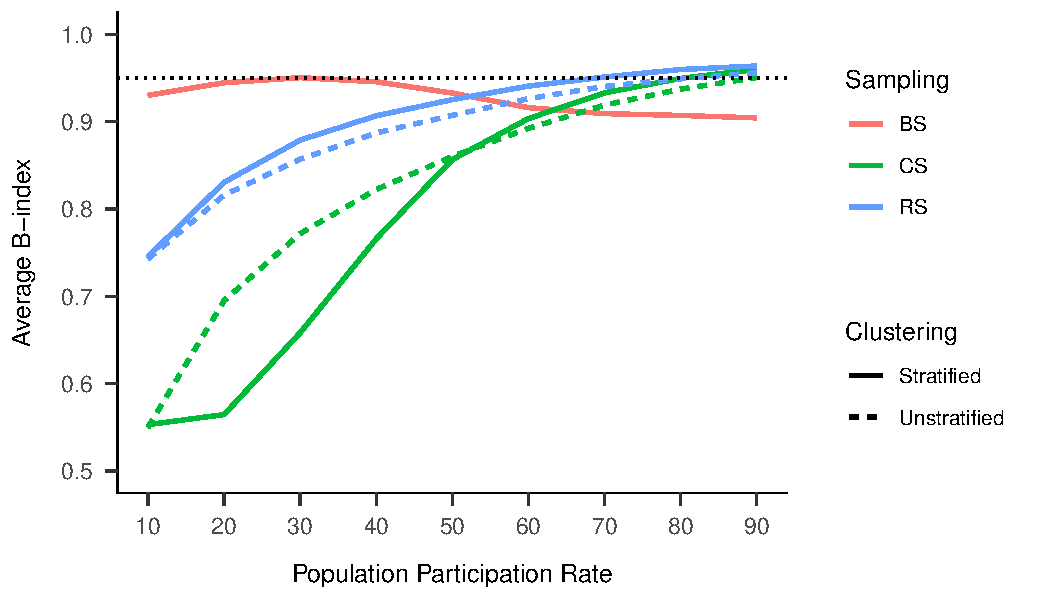
\includegraphics{GenSamp-Paper_files/figure-latex/fig-avg-Bindex-1.pdf}
\caption{\label{fig:fig-avg-Bindex}Averge \(B\)-index for varying participation rates, by sampling method. Horizontal dotted line represented index of .95 indicating a high level of generalizability.}
\end{figure}

\hypertarget{stratification-versus-participation}{%
\subsubsection{Stratification Versus Participation}\label{stratification-versus-participation}}

One potential explanation for why stratification may underperform in certain circumstances is if the strata do not explain any variance in a covariate that is related to participation. To examin this we calculated the ICC for each covariate across strata and compared it to the covariates log-odds coeficient in the participation response model. Table \ref{fig:tab-ICC-Pars} displays these values.

\begin{table}[tbp]
\begin{center}
\begin{threeparttable}
\caption{\label{tab:tab-ICC-Pars}Odds ratio coeficients and strata ICC}
\begin{tabular}{llll}
\toprule
Variables & ICC & RGM Coeficient & Quality\\
\midrule
\% White & 0.67 & 0.54 & Very Good\\
District Size & 0.12 & 0.52 & Very Good\\
Schoolwide Title I & 0.94 & 0.02 & Good\\
\% F/RL & 0.76 & 0.08 & Good\\
Urban & 0.91 & 0.43 & Good\\
Town/Rural & 0.27 & 0.40 & Good\\
\% Hispanic & 0.66 & 0.40 & Good\\
\% ELL & 0.54 & 0.41 & Good\\
\% Female & 0.00 & 0.02 & Neutral\\
Students/Teachers & 0.10 & 0.10 & Neutral\\
N Students & 0.06 & 0.37 & Bad\\
Suburban & 0.58 & 0.01 & Bad\\
\% Black & 0.06 & 0.29 & Bad\\
\bottomrule
\end{tabular}
\end{threeparttable}
\end{center}
\end{table}

\hypertarget{standardized-mean-differences}{%
\subsubsection{Standardized Mean Differences}\label{standardized-mean-differences}}

Figure \ref{fig:fig-SMD-by-Var-example} displays the average SMD between the samples and the population for four covariates and at each population participation rate resulting from each sampling method. The dotted horizontal line indicates a cutoff of .25, where SMDs above that indicate large differences between the sample and population for that covariate. For 8 out of the 13 covariates, stratified methods consistently performed better than unstratified methods. For 2 covariates (percent female and student to teacher ratio) all methods resulted in acceptible SMDs. For 3 covariates (percent black, suburban schools, and school size) the unstratified methods performed better than their stratified counterparts. SBS generally performed as well as or better than SRS. URS often resulted in highly unrepresentative samples except in cases where population participation rates were extremely high.







\begin{figure}
\centering
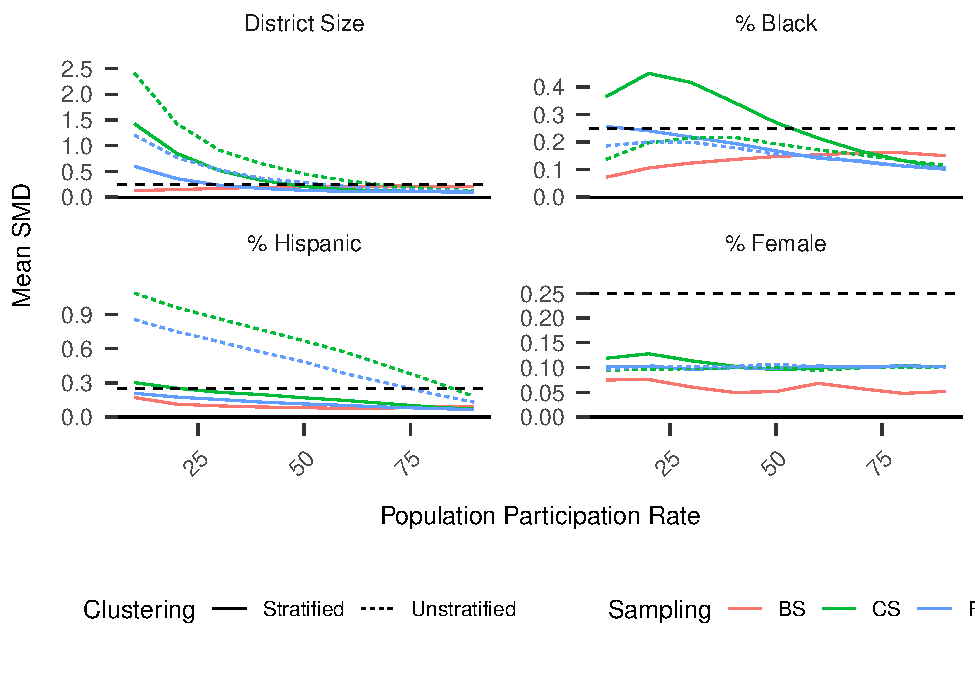
\includegraphics{GenSamp-Paper_files/figure-latex/fig-SMD-by-Var-example-1.pdf}
\caption{\label{fig:fig-SMD-by-Var-example}Averge Standardized Mean Differences between sample and population for select covariates}
\end{figure}

\hypertarget{feasibility-1}{%
\subsection{Feasibility}\label{feasibility-1}}

Figure \ref{fig:fig-units-contacted} reports the average number of schools that needed to be contacted before a full sample of \(N = 60\) schools was selected. At higher response rates differences between methods were negligible. However, as response rates decreased the disparity between the methods became more apparent. Overall, UCS required the least \enquote{effort} to recruit a full sample, followed by URS and SCS, SRS, and finally SBS. Figure \ref{fig:fig-response-rates} plots the response rates of schools approached for recruitment against the population response rates. As expected, URS response rates reflected those in the population. Both UCS and SCS resulted in higher response rates, while SRS and SBS resulted in lower response rates.





\begin{figure}
\centering
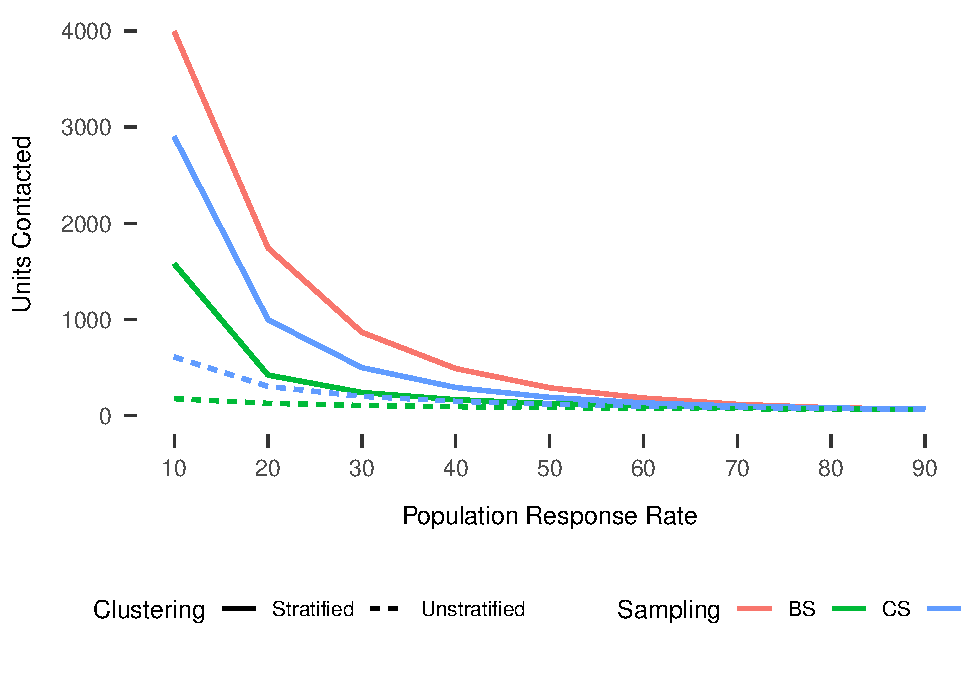
\includegraphics{GenSamp-Paper_files/figure-latex/fig-units-contacted-1.pdf}
\caption{\label{fig:fig-units-contacted}Averge number of schools contacted to achieve \(N = 60\)}
\end{figure}



\begin{figure}
\centering
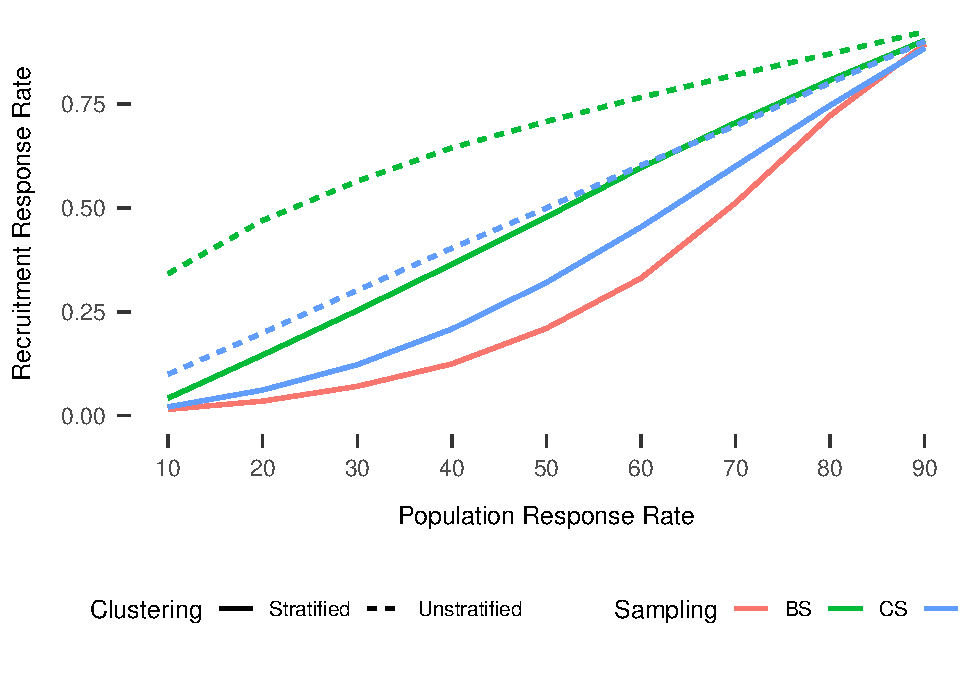
\includegraphics{GenSamp-Paper_files/figure-latex/fig-response-rates-1.pdf}
\caption{\label{fig:fig-response-rates}Recruitment response rates for each sampling method}
\end{figure}

\newpage

\hypertarget{discussion}{%
\section{Discussion}\label{discussion}}

The main goal of this study was to lay the groundwork for exploring the effectiveness and feasibility of sampling methods in the educational context. In terms of selecting a generalizable sample, SBS resulted in a considerable improvement compared to UCS. However, given the difficulty with which those samples are recruited, SBS is unlikely to be fully implemented in the ideal form. Instead, SCS may be a reasonable compromise. Our findings indicate that any sampling method is greatly improved by first stratifying the population. We show that, in certain cases, performing a convenience sample within strata (SCS) is comparable to simple random sampling (URS) both in terms of generalizability and feasibility.

An exception to this seems to be driven largely by the accuracy of the clustering method with respect to the response model. For instance, in Figure \ref{fig:fig-SMD-by-Var-example} we see that all methods of sampling result in balance on percentage of Black students, except for stratfied convenience sampling. This is likely a result of the covariate having a strong relationship with participation, but not being weighed enough in the cluster analysis during stratification. Table \ref{tab:tab-ICC-Pars} displays the calculated intraclass correlation coeficient (ICC) for each covariate along the strata, and the coeficient for each covariate in the response generating model. For covariates where one value (ICC or coeficient) is high, while the other is low, stratified sampling techniques resulted in poor balance as presented in figure \ref{fig:fig-SMD-by-Var-bad}

URS is considered the gold standard for generalizabilty, however it is not typically implemented due to it requiring substantial resources and other concerns of practicality. The advantage of SCS here is that it enables researchers to mitigate recruitment costs by targeting schools from the same strata that are in close proximity to each other. Beyond generalizability, stratifying in this manner also offers the additional advantage of transparency by forcing the researcher to make sampling decisions in the study design phase, and to keep track of sampling decisions as recruitment is implemented.

Our work uncovered several limitations in designing sampling and participation models. The sampling methods we developed made several assumptions about researcher and recruiter behavior in selecting a sample. First, that recruiters always prioritize schools that are most likely to participate. In truth, many other factors play a role such as proximity of sample sites to the researcher and to each other, existing relationships between the recruiters and the sample sites, and other researcher assumptions about the sample site's characteristics. Second, that recruiters have approximate knowledge of how likely a sampled site is to participate. Though researchers may speculate about sites that are more willing to participate (schools in larger urban districts) and prioritize recruiting such sites, it is not likely that they would estimate willingness as well as we have simulated. Given this, it is possible that the \enquote{feasibility} of the convenience methods is overestimated.



\begin{figure}
\centering
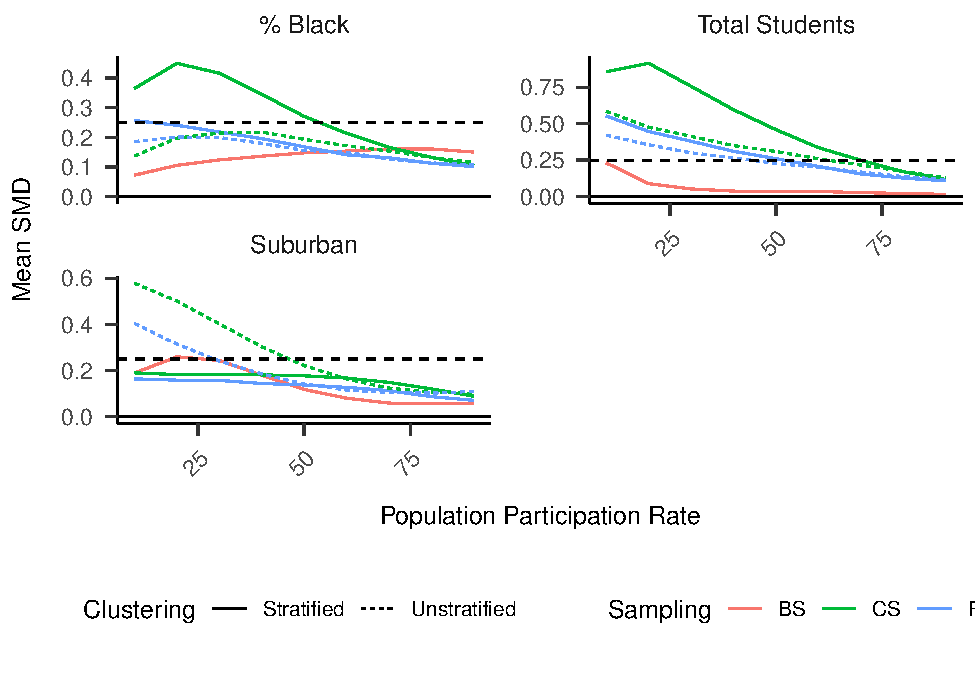
\includegraphics{GenSamp-Paper_files/figure-latex/fig-SMD-by-Var-bad-1.pdf}
\caption{\label{fig:fig-SMD-by-Var-bad}Poor balance for stratfied methods}
\end{figure}

Our participation model is also speculative. The parameters in our response generating model are based on values from a study that examined the difference between schools participating in large-scale randomized control trials (RCT) and the overall population of schools. However, these RCTs themselves typically rely on some form of convenience sampling. In that sense our parameters reflect participation rates of schools that are likely to participate in RCTs, rather than the full population of schools. Furthermore, the decision of whether a school participates in such a study is multi-leveled. Generally, districts serve as gatekeepers, requiring research requests to be submitted and approved before recruitment can begin. If the request is denied, no schools within that district may be recruited. If approved, schools may be contacted individually. The ultimate decision may then rest with administrators, or they may be passed on to teachers most affected by the study. Despite these limitations, we believe that our findings reasonably represent the relative performance of the various sampling methods we tested in the context of educational research.

Finally, we hope to make clear the disadvantages of convenience sampling in this context. Large scale MRTs are expensive to implement, however by not investing in robust recruitment strategies researchers severely limit the impact and relevance of of their work. We believe that the increased cost of a sampling method designed for generalizability is greatly outweighed by the benefit of an intervention whose impacts we can estimate more accurately and for a wider population.

\hypertarget{references}{%
\section{References}\label{references}}

\begingroup
\setlength{\parindent}{-0.5in}
\setlength{\leftskip}{0.5in}

\hypertarget{refs}{}
\leavevmode\hypertarget{ref-calinskiDendriteMethodCluster1974}{}%
Cali\a'nski, T., \& Harabasz, J. (1974). A dendrite method for cluster analysis. \emph{Communications in Statistics}, \emph{3}(1), 1--27. \url{https://doi.org/10.1080/03610927408827101}

\leavevmode\hypertarget{ref-fellersDevelopingApproachDetermine2017}{}%
Fellers, L. (2017). \emph{Developing an approach to determine generalizability: A review of efficacy and effectiveness trials funded by the Institute of Education Sciences} (Ph.D.). Columbia University, United States -- New York. Retrieved from \url{https://search.proquest.com/docview/1865595768/abstract/40FD82F4A0C24535PQ/1}

\leavevmode\hypertarget{ref-gowerGeneralCoefficientSimilarity1971}{}%
Gower, J. C. (1971). A General Coefficient of Similarity and Some of Its Properties. \emph{Biometrics}, \emph{27}(4), 857--871. \url{https://doi.org/10.2307/2528823}

\leavevmode\hypertarget{ref-grovesSurveyMethodology2004}{}%
Groves, R. M. (Ed.). (2004). \emph{Survey methodology}. Hoboken, N.J: Wiley-Interscience.

\leavevmode\hypertarget{ref-hennigHowFindAppropriate2013}{}%
Hennig, C., \& Liao, T. F. (2013). How to find an appropriate clustering for mixed-type variables with application to socio-economic stratification: How to Find an Appropriate Clustering. \emph{Journal of the Royal Statistical Society: Series C (Applied Statistics)}, \emph{62}(3), 309--369. \url{https://doi.org/10.1111/j.1467-9876.2012.01066.x}

\leavevmode\hypertarget{ref-kernAssessingMethodsGeneralizing2016}{}%
Kern, H. L., Stuart, E. A., Hill, J., \& Green, D. P. (2016). Assessing Methods for Generalizing Experimental Impact Estimates to Target Populations. \emph{Journal of Research on Educational Effectiveness}, \emph{9}(1), 103--127. \url{https://doi.org/10.1080/19345747.2015.1060282}

\leavevmode\hypertarget{ref-olsenExternalValidityPolicy2013}{}%
Olsen, R. B., Orr, L. L., Bell, S. H., \& Stuart, E. A. (2013). External Validity in Policy Evaluations That Choose Sites Purposively. \emph{Journal of Policy Analysis and Management}, \emph{32}(1), 107--121. \url{https://doi.org/10.1002/pam.21660}

\leavevmode\hypertarget{ref-omuircheartaighGeneralizingUnrepresentativeExperiments2014}{}%
O'Muircheartaigh, C., \& Hedges, L. V. (2014). Generalizing from unrepresentative experiments: A stratified propensity score approach. \emph{Journal of the Royal Statistical Society: Series C (Applied Statistics)}, \emph{63}(2), 195--210. \url{https://doi.org/10.1111/rssc.12037}

\leavevmode\hypertarget{ref-raudenbushStatisticalPowerOptimal2000}{}%
Raudenbush, S. W., \& Liu, X. (2000). Statistical power and optimal design for multisite randomized trials. \emph{Psychological Methods}, \emph{5}(2), 199--213. \url{https://doi.org/10.1037//1082-989X.5.2.199}

\leavevmode\hypertarget{ref-roschelleIntegrationTechnologyCurriculum2010}{}%
Roschelle, J., Shechtman, N., Tatar, D., Hegedus, S., Hopkins, B., Empson, S., \ldots{} Gallagher, L. P. (2010). Integration of Technology, Curriculum, and Professional Development for Advancing Middle School Mathematics: Three Large-Scale Studies. \emph{American Educational Research Journal}, \emph{47}(4), 833--878.

\leavevmode\hypertarget{ref-shadishExperimentalQuasiexperimentalDesigns2002}{}%
Shadish, W. R., Cook, T. D., \& Campbell, D. T. (2002). \emph{Experimental and quasi-experimental designs for generalized causal inference}. Boston, MA, US: Houghton, Mifflin and Company.

\leavevmode\hypertarget{ref-steinleyKmeansClusteringHalfcentury2006}{}%
Steinley, D. (2006). K-means clustering: A half-century synthesis. \emph{British Journal of Mathematical and Statistical Psychology}, \emph{59}(1), 1--34. \url{https://doi.org/10.1348/000711005X48266}

\leavevmode\hypertarget{ref-stuartCharacteristicsSchoolDistricts2017}{}%
Stuart, E. A., Bell, S. H., Ebnesajjad, C., Olsen, R. B., \& Orr, L. L. (2017). Characteristics of School Districts That Participate in Rigorous National Educational Evaluations. \emph{Journal of Research on Educational Effectiveness}, \emph{10}(1), 168--206. \url{https://doi.org/10.1080/19345747.2016.1205160}

\leavevmode\hypertarget{ref-stuartUsePropensityScores2011}{}%
Stuart, E. A., Cole, S. R., Bradshaw, C. P., \& Leaf, P. J. (2011). The use of propensity scores to assess the generalizability of results from randomized trials: Use of Propensity Scores to Assess Generalizability. \emph{Journal of the Royal Statistical Society: Series A (Statistics in Society)}, \emph{174}(2), 369--386. \url{https://doi.org/10.1111/j.1467-985X.2010.00673.x}

\leavevmode\hypertarget{ref-tiptonImprovingGeneralizationsExperiments2013}{}%
Tipton, E. (2013a). Improving Generalizations From Experiments Using Propensity Score Subclassification: Assumptions, Properties, and Contexts. \emph{Journal of Educational and Behavioral Statistics}, \emph{38}(3), 239--266. Retrieved from \url{https://www.jstor.org/stable/41999424}

\leavevmode\hypertarget{ref-tiptonStratifiedSamplingUsing2013}{}%
Tipton, E. (2013b). Stratified Sampling Using Cluster Analysis: A Sample Selection Strategy for Improved Generalizations From Experiments. \emph{Evaluation Review}, \emph{37}(2), 109--139. \url{https://doi.org/10.1177/0193841X13516324}

\leavevmode\hypertarget{ref-tiptonHowGeneralizableYour2014}{}%
Tipton, E. (2014). How Generalizable Is Your Experiment? An Index for Comparing Experimental Samples and Populations. \emph{Journal of Educational and Behavioral Statistics}, \emph{39}(6), 478--501.

\leavevmode\hypertarget{ref-tiptonSiteSelectionExperiments2016}{}%
Tipton, E., Fellers, L., Caverly, S., Vaden-Kiernan, M., Borman, G., Sullivan, K., \& de Castilla, V. R. (2016). Site Selection in Experiments: An Assessment of Site Recruitment and Generalizability in Two Scale-up Studies. \emph{Journal of Research on Educational Effectiveness}, \emph{9}(sup1), 209--228. \url{https://doi.org/10.1080/19345747.2015.1105895}

\leavevmode\hypertarget{ref-tiptonImplicationsSmallSamples2017}{}%
Tipton, E., Hallberg, K., Hedges, L. V., \& Chan, W. (2017). Implications of Small Samples for Generalization: Adjustments and Rules of Thumb. \emph{Evaluation Review}, \emph{41}(5), 472--505. \url{https://doi.org/10.1177/0193841X16655665}

\endgroup


\end{document}
